\documentclass{article}

% Bibliography
\usepackage{natbib}
\bibpunct{(}{)}{;}{a}{}{;}

% Use 'It was found that A is B (Name 1234)' style
\setcitestyle{authoryear,open={},close={}}

% Affiliations
\usepackage{authblk}
\title{The error when inferring phylogenies with incipient species by a Birth-Death model}
% \subtitle{Should protracted speciation be incorporated in phylogenetic tree construction methods?}

\author[1]{Rich\`el J.C. Bilderbeek}
\author[1]{Rampal S. Etienne}
\affil[1]{Groningen Institute for Evolutionary Life Sciences, University of Groningen, Groningen, The Netherlands}

% Load my functions
% The functions used

% My first function, kept for nostalic reasons
\newcommand{\sayhello}{hello and howdy!}

% Making a note
\newcommand\note[1]{\textcolor{green}{\todo{#1}}}

% From https://tex.stackexchange.com/a/98034
\newcommand*\mean[1]{\overline{#1}}

% From https://tex.stackexchange.com/a/101138
% \newcommand\reallywidetilde[1]{\ThisStyle{%
%   \setbox0=\hbox{$\SavedStyle#1$}%
%   \stackengine{-.1\LMpt}{$\SavedStyle#1$}{%
%     \stretchto{\scaleto{\SavedStyle\mkern.2mu\AC}{.5150\wd0}}{.6\ht0}%
%   }{O}{c}{F}{T}{S}%
% }}

% Adapted from 'mean', use 'reallywidetilde'
% \newcommand*\median[1]{\reallywidetilde{#1}}

\newcommand*\median[1]{\widetilde{#1}}

%%%%%%%%%%%%%%%%%%%%%%%%%%%%%%%%%%%%%%%%%%%%%%%%%%%%%%%%%%%%%%%%%%%%%%%%%%%%%%%%
% Create the TikZ picture for fig:experiment
%%%%%%%%%%%%%%%%%%%%%%%%%%%%%%%%%%%%%%%%%%%%%%%%%%%%%%%%%%%%%%%%%%%%%%%%%%%%%%%%
\newcommand{\CreateTikzFigureExperiment} {

  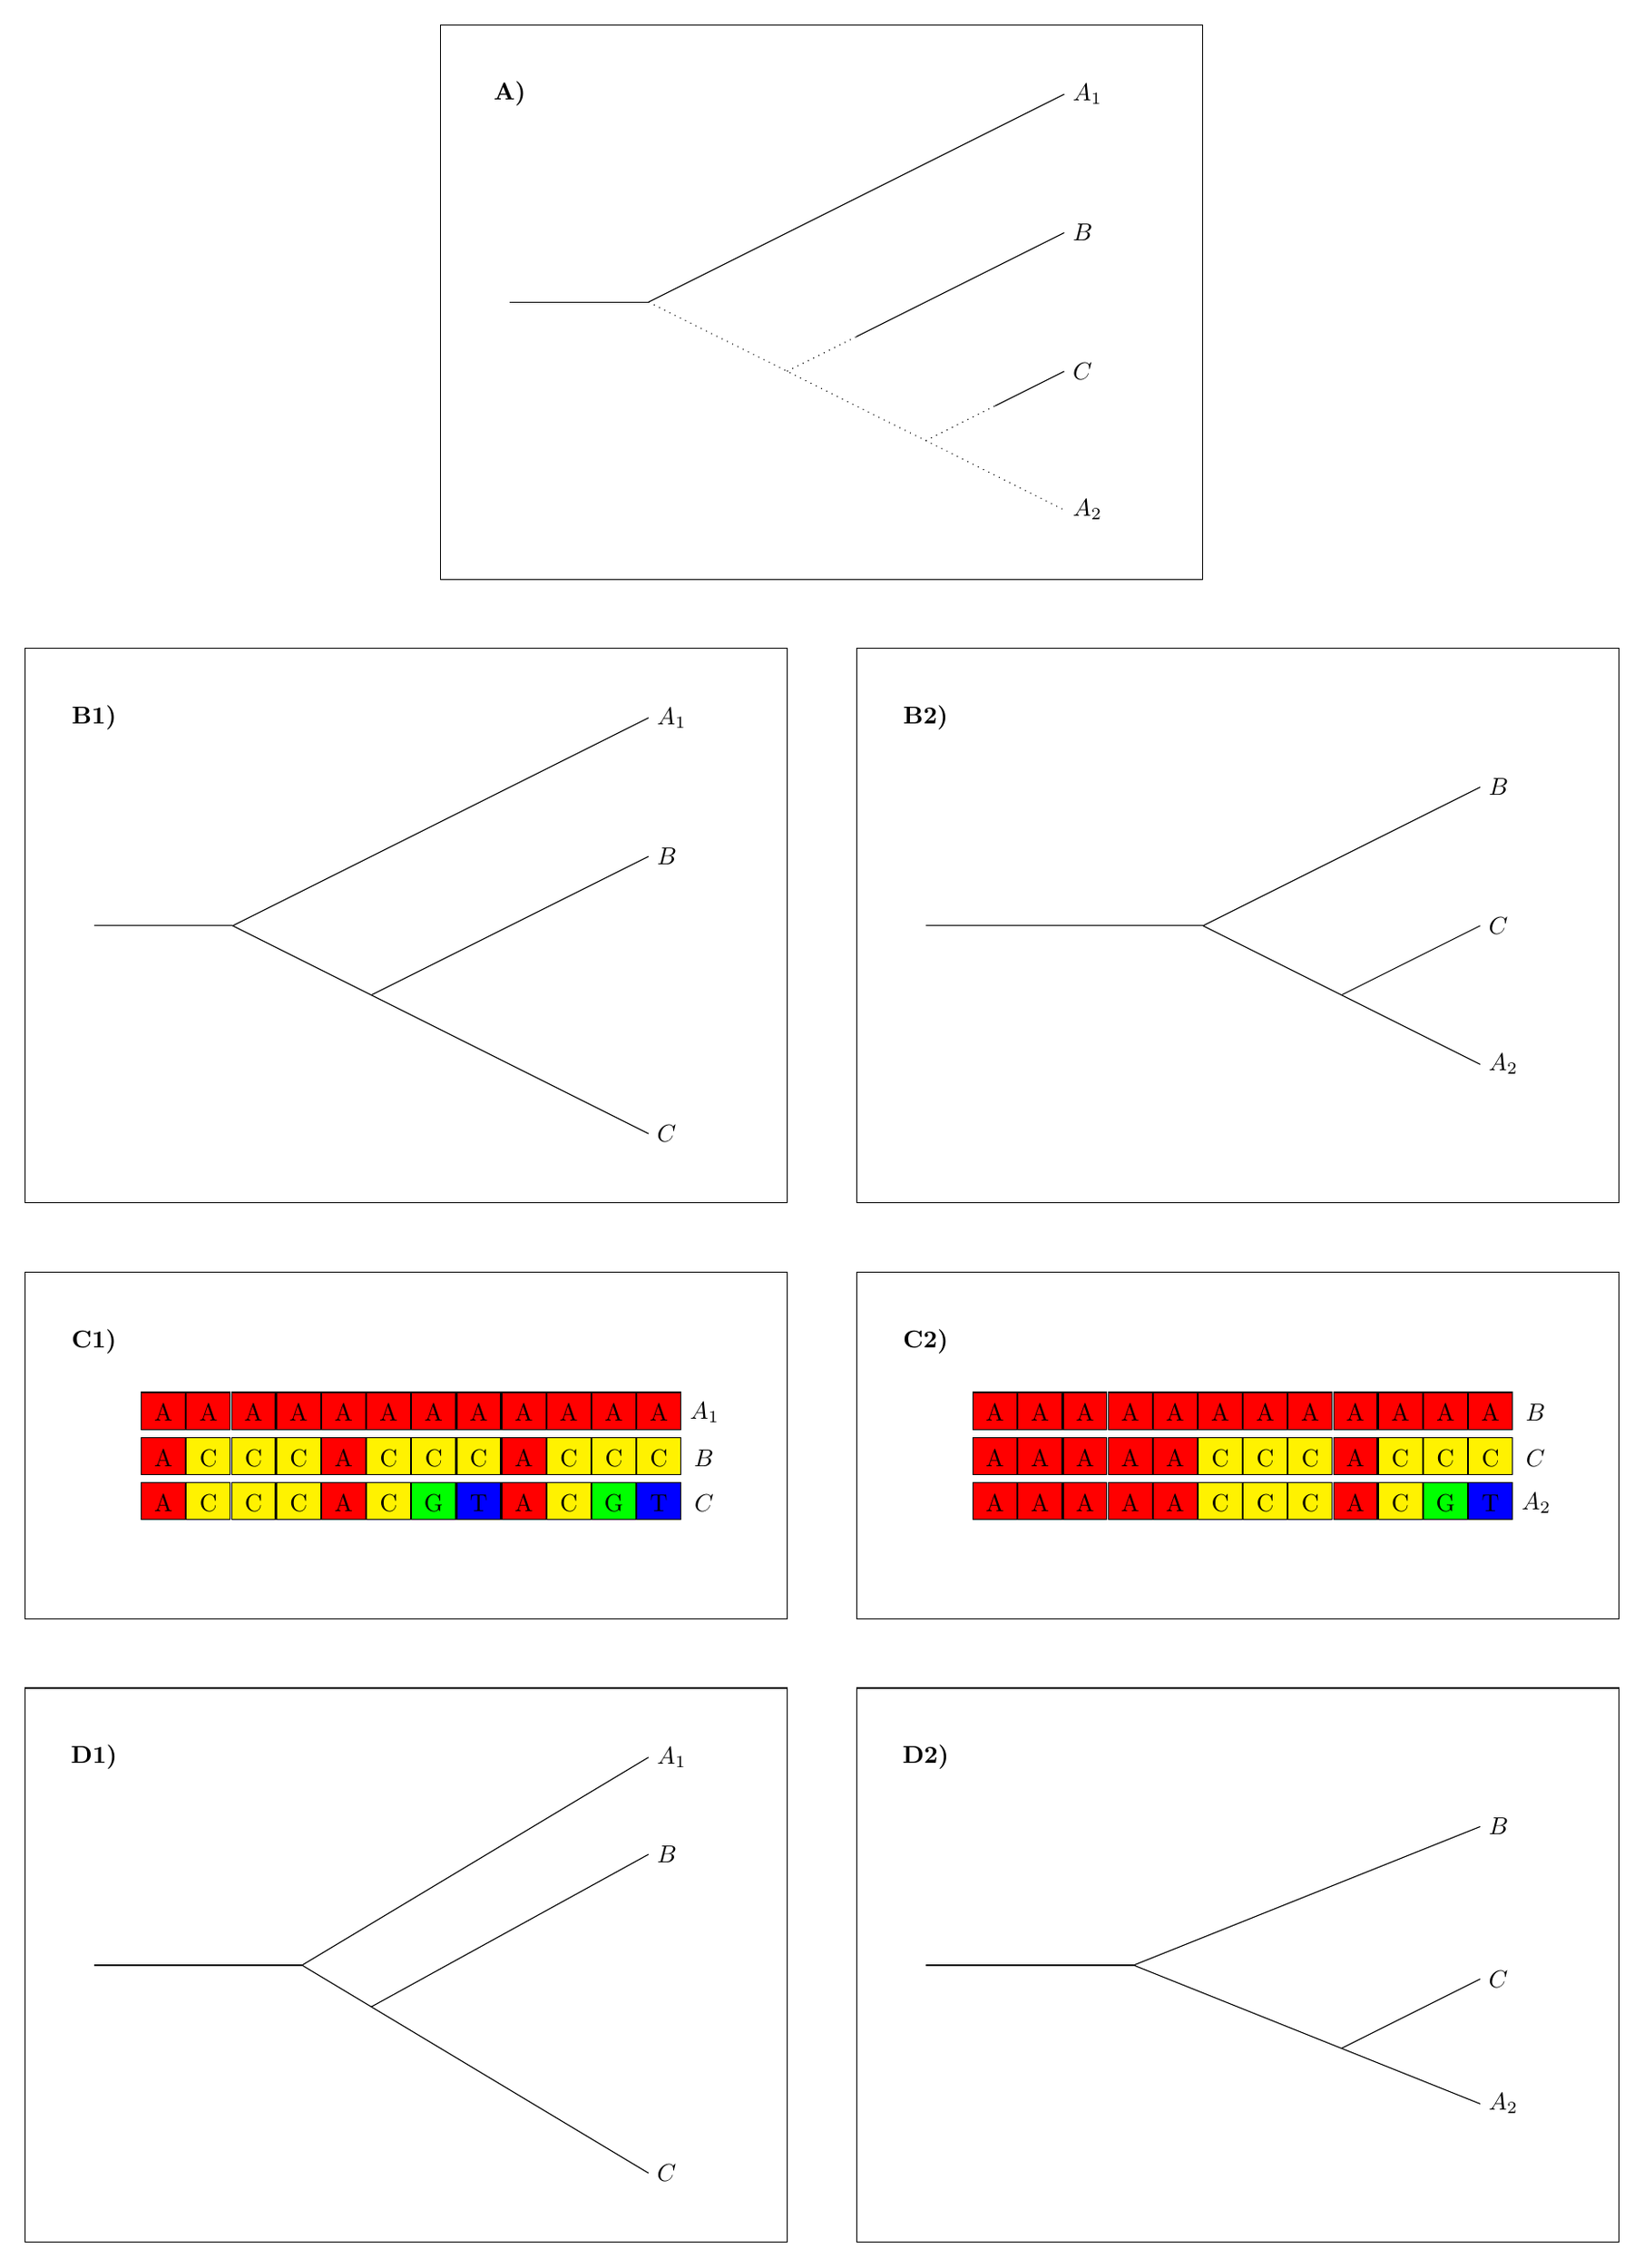
\begin{tikzpicture} 

    % Incipient species tree
    \begin{scope}[shift={(0,0)}] 

      \node[font = \bf] at (0, 0) {A)};
      \draw (-1,1) rectangle (10,-7);

      % Drawing of the phylogeny
      \begin{scope}[shift={(0,-3)}] 
        \draw (0, 0) -- (2,  0); % stem 
        \draw (2, 0) -- (8,  3) node[anchor=west] {$A_1$};
        \draw[dotted] (4,  -1) -- (5, -0.5); \draw (5, -0.5) -- (8, 1) node[anchor=west] {$B$};
        \draw[dotted] (6,  -2) -- (7, -1.5); \draw (7, -1.5) -- (8, -1) node[anchor=west] {$C$};
        \draw[dotted] (2,0) -- (8, -3) node[anchor=west] {$A_2$};
      \end{scope} % Drawing of the phylogeny

    \end{scope}


    % Species tree, oldest
    \begin{scope}[shift={(-6,-9)}] 

      \node[font = \bf] at (0.0, 0  ) {B1)};
      \draw (-1,1) rectangle (10,-7);

      % Drawing of the species tree, oldest
      \begin{scope}[shift={(0,-3)}] 
        \draw (0, 0) -- (2,  0); % stem 
        \draw (2, 0) -- (8,  3) node[anchor=west] {$A_1$};
        \draw (4,  -1) -- (8, 1) node[anchor=west] {$B$};
        \draw (2,0) -- (8, -3) node[anchor=west] {$C$};
      \end{scope} % Drawing of the species tree, oldest

    \end{scope}


    % Species tree, youngest
    \begin{scope}[shift={( 6,-9)}] 

      \node[font = \bf] at (0, 0) {B2)};
      \draw (-1,1) rectangle (10,-7);

      % Drawing of the species tree, youngest
      \begin{scope}[shift={(0,-3)}] 
        \draw (0, 0) -- (4,  0); % stem 
        \draw (4, 0) -- (8,  2) node[anchor=west] {$B$};
        \draw (6,-1) -- (8,  0) node[anchor=west] {$C$};
        \draw (4, 0) -- (8, -2) node[anchor=west] {$A_2$};
      \end{scope} % Drawing of the species tree, youngest

    \end{scope}

    % Alignment, oldest
    \begin{scope}[shift={(-6,-18)}] 

      \node[font = \bf] at (0.0, 0  ) {C1)};
      \draw (-1,1) rectangle (10,-4);

      % Drawing of the alignment
      \begin{scope}[shift={(1,-1)}, text width = 4mm, text height = 3mm, align = center, scale = 1.3] 

        \node[draw, fill = red   ] at (0.0, 0  ) {A};
        \node[draw, fill = red   ] at (0.5, 0  ) {A};
        \node[draw, fill = red   ] at (1.0, 0  ) {A};
        \node[draw, fill = red   ] at (1.5, 0  ) {A};
        \node[draw, fill = red   ] at (2.0, 0  ) {A};
        \node[draw, fill = red   ] at (2.5, 0  ) {A};
        \node[draw, fill = red   ] at (3.0, 0  ) {A};
        \node[draw, fill = red   ] at (3.5, 0  ) {A};
        \node[draw, fill = red   ] at (4.0, 0  ) {A};
        \node[draw, fill = red   ] at (4.5, 0  ) {A};
        \node[draw, fill = red   ] at (5.0, 0  ) {A};
        \node[draw, fill = red   ] at (5.5, 0  ) {A};
        \node[                   ] at (6.0, 0  ) {$A_1$};

        \node[draw, fill = red   ] at (0.0, -0.5) {A};
        \node[draw, fill = yellow] at (0.5, -0.5) {C};
        \node[draw, fill = yellow] at (1.0, -0.5) {C};
        \node[draw, fill = yellow] at (1.5, -0.5) {C};
        \node[draw, fill = red   ] at (2.0, -0.5) {A};
        \node[draw, fill = yellow] at (2.5, -0.5) {C};
        \node[draw, fill = yellow] at (3.0, -0.5) {C};
        \node[draw, fill = yellow] at (3.5, -0.5) {C};
        \node[draw, fill = red   ] at (4.0, -0.5) {A};
        \node[draw, fill = yellow] at (4.5, -0.5) {C};
        \node[draw, fill = yellow] at (5.0, -0.5) {C};
        \node[draw, fill = yellow] at (5.5, -0.5) {C};
        \node[                   ] at (6.0, -0.5) {$B$};

        \node[draw, fill = red] at (0.0, -1.0) {A};
        \node[draw, fill = yellow] at (0.5, -1.0) {C};
        \node[draw, fill = yellow] at (1.0, -1.0) {C};
        \node[draw, fill = yellow] at (1.5, -1.0) {C};
        \node[draw, fill = red   ] at (2.0, -1.0) {A};
        \node[draw, fill = yellow] at (2.5, -1.0) {C};
        \node[draw, fill = green ] at (3.0, -1.0) {G};
        \node[draw, fill = blue  ] at (3.5, -1.0) {T};
        \node[draw, fill = red   ] at (4.0, -1.0) {A};
        \node[draw, fill = yellow] at (4.5, -1.0) {C};
        \node[draw, fill = green ] at (5.0, -1.0) {G};
        \node[draw, fill = blue  ] at (5.5, -1.0) {T};
        \node[                   ] at (6.0, -1.0) {$C$};

      \end{scope} % Drawing of the alignment

    \end{scope}

    % Alignment, youngest
    \begin{scope}[shift={(6,-18)}] 

      \node[font = \bf] at (0.0, 0  ) {C2)};
      \draw (-1,1) rectangle (10,-4);

      % Drawing of the alignment
      \begin{scope}[shift={(1,-1)}, text width = 4mm, text height = 3mm, align = center, scale = 1.3] 

        \node[draw, fill = red   ] at (0.0, 0  ) {A};
        \node[draw, fill = red   ] at (0.5, 0  ) {A};
        \node[draw, fill = red   ] at (1.0, 0  ) {A};
        \node[draw, fill = red   ] at (1.5, 0  ) {A};
        \node[draw, fill = red   ] at (2.0, 0  ) {A};
        \node[draw, fill = red   ] at (2.5, 0  ) {A};
        \node[draw, fill = red   ] at (3.0, 0  ) {A};
        \node[draw, fill = red   ] at (3.5, 0  ) {A};
        \node[draw, fill = red   ] at (4.0, 0  ) {A};
        \node[draw, fill = red   ] at (4.5, 0  ) {A};
        \node[draw, fill = red   ] at (5.0, 0  ) {A};
        \node[draw, fill = red   ] at (5.5, 0  ) {A};
        \node[                   ] at (6.0, 0  ) {$B$};

        \node[draw, fill = red   ] at (0.0, -0.5) {A};
        \node[draw, fill = red   ] at (0.5, -0.5) {A};
        \node[draw, fill = red   ] at (1.0, -0.5) {A};
        \node[draw, fill = red   ] at (1.5, -0.5) {A};
        \node[draw, fill = red   ] at (2.0, -0.5) {A};
        \node[draw, fill = yellow] at (2.5, -0.5) {C};
        \node[draw, fill = yellow] at (3.0, -0.5) {C};
        \node[draw, fill = yellow] at (3.5, -0.5) {C};
        \node[draw, fill = red   ] at (4.0, -0.5) {A};
        \node[draw, fill = yellow] at (4.5, -0.5) {C};
        \node[draw, fill = yellow] at (5.0, -0.5) {C};
        \node[draw, fill = yellow] at (5.5, -0.5) {C};
        \node[                   ] at (6.0, -0.5) {$C$};

        \node[draw, fill = red   ] at (0.0, -1.0) {A};
        \node[draw, fill = red   ] at (0.5, -1.0) {A};
        \node[draw, fill = red   ] at (1.0, -1.0) {A};
        \node[draw, fill = red   ] at (1.5, -1.0) {A};
        \node[draw, fill = red   ] at (2.0, -1.0) {A};
        \node[draw, fill = yellow] at (2.5, -1.0) {C};
        \node[draw, fill = yellow] at (3.0, -1.0) {C};
        \node[draw, fill = yellow] at (3.5, -1.0) {C};
        \node[draw, fill = red   ] at (4.0, -1.0) {A};
        \node[draw, fill = yellow] at (4.5, -1.0) {C};
        \node[draw, fill = green ] at (5.0, -1.0) {G};
        \node[draw, fill = blue  ] at (5.5, -1.0) {T};
        \node[                   ] at (6.0, -1.0) {$A_2$};

      \end{scope} % Drawing of the alignment

    \end{scope}



    % Estimated species tree, oldest
    \begin{scope}[shift={(-6,-24)}] 

      \node[font = \bf] at (0, 0) {D1)};
      \draw (-1,1) rectangle (10,-7);

      \begin{scope}[shift={(0,-3)}] 
        \draw (0, 0) -- (3,  0);
        \draw (3, 0) -- (8, 3) node[anchor=west] {$A_1$};
        \draw (4,-0.6) -- (8, 1.6) node[anchor=west] {$B$};
        \draw (3, 0) -- (8,-3) node[anchor=west] {$C$};
      \end{scope}

    \end{scope}


    % Estimated species tree, youngest
    \begin{scope}[shift={(6,-24)}] 

      \node[font = \bf] at (0, 0) {D2)};
      \draw (-1,1) rectangle (10,-7);

      \begin{scope}[shift={(0,-3)}] 
        \draw (0, 0) -- (3,  0);
        \draw (3, 0) -- (8,  2) node[anchor=west] {$B$};
        \draw (6,-1.2) -- (8, -0.2) node[anchor=west] {$C$};
        \draw (3, 0) -- (8, -2) node[anchor=west] {$A_2$};
      \end{scope}

    \end{scope}

  \end{tikzpicture}
} % End of create_figure_experiment definition
%%%%%%%%%%%%%%%%%%%%%%%%%%%%%%%%%%%%%%%%%%%%%%%%%%%%%%%%%%%%%%%%%%%%%%%%%%%%%%%%




%%%%%%%%%%%%%%%%%%%%%%%%%%%%%%%%%%%%%%%%%%%%%%%%%%%%%%%%%%%%%%%%%%%%%%%%%%%%%%%%
% Create the TikZ picture of fig:sampling
%%%%%%%%%%%%%%%%%%%%%%%%%%%%%%%%%%%%%%%%%%%%%%%%%%%%%%%%%%%%%%%%%%%%%%%%%%%%%%%%
\newcommand{\CreateTikzFigureSampling} {

  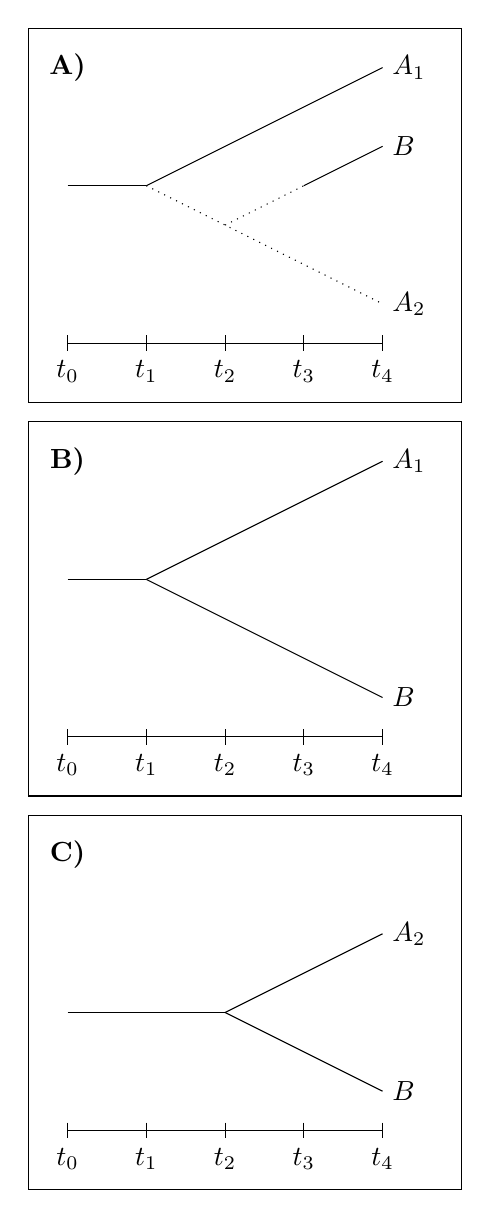
\begin{tikzpicture}[scale = 0.5] 

    \begin{scope}[shift={(0,0)}] 

      \node[font = \bf] at (0, 0) {A)};
      \draw (-1,1) rectangle (10,-8.5);

      % Drawing of the phylogeny
      \begin{scope}[shift={(0,-3)}] 
        \draw (0, 0) -- (2,  0);
        \draw (2, 0) -- (8,  3) node[anchor=west] {$A_1$};
        \draw[dotted] (2, 0) -- (8, -3) node[anchor=west] {$A_2$};
        \draw[dotted] (4, -1) -- (6, 0);
        \draw (6, 0) -- (8, 1) node[anchor=west] {$B$};
        % time scale
        \draw (0, -4) -- (8,  -4);
        \draw (0, -3.8) -- (0,  -4.2) node[anchor=north] {$t_0$};
        \draw (2, -3.8) -- (2,  -4.2) node[anchor=north] {$t_1$};
        \draw (4, -3.8) -- (4,  -4.2) node[anchor=north] {$t_2$};
        \draw (6, -3.8) -- (6,  -4.2) node[anchor=north] {$t_3$};
        \draw (8, -3.8) -- (8,  -4.2) node[anchor=north] {$t_4$};
      \end{scope} % Drawing of the phylogeny

    \end{scope}
    \begin{scope}[shift={(0, -10)}] 

      \node[font = \bf] at (0, 0) {B)};
      \draw (-1,1) rectangle (10,-8.5);

      % Drawing of the phylogeny
      \begin{scope}[shift={(0,-3)}] 
        \draw (0, 0) -- (2,  0);
        \draw (2, 0) -- (8,  3) node[anchor=west] {$A_1$};
        \draw (2, 0) -- (8, -3) node[anchor=west] {$B$};
        % time scale
        \draw (0, -4) -- (8,  -4);
        \draw (0, -3.8) -- (0,  -4.2) node[anchor=north] {$t_0$};
        \draw (2, -3.8) -- (2,  -4.2) node[anchor=north] {$t_1$};
        \draw (4, -3.8) -- (4,  -4.2) node[anchor=north] {$t_2$};
        \draw (6, -3.8) -- (6,  -4.2) node[anchor=north] {$t_3$};
        \draw (8, -3.8) -- (8,  -4.2) node[anchor=north] {$t_4$};
      \end{scope} % Drawing of the phylogeny

    \end{scope}
    \begin{scope}[shift={(0,-20)}] 

      \node[font = \bf] at (0, 0) {C)};
      \draw (-1,1) rectangle (10,-8.5);

      % Drawing of the phylogeny
      \begin{scope}[shift={(0,-3)}] 
        \draw (0, -1) -- (4, -1) ;
        \draw (4, -1) -- (8, -3) node[anchor=west] {$B$};
        \draw (4, -1) -- (8,  1) node[anchor=west] {$A_2$};
        % time scale
        \draw (0, -4) -- (8,  -4);
        \draw (0, -3.8) -- (0,  -4.2) node[anchor=north] {$t_0$};
        \draw (2, -3.8) -- (2,  -4.2) node[anchor=north] {$t_1$};
        \draw (4, -3.8) -- (4,  -4.2) node[anchor=north] {$t_2$};
        \draw (6, -3.8) -- (6,  -4.2) node[anchor=north] {$t_3$};
        \draw (8, -3.8) -- (8,  -4.2) node[anchor=north] {$t_4$};
      \end{scope} % Drawing of the phylogeny

    \end{scope}
  \end{tikzpicture}

} % End of create_figure_experiment definition
%%%%%%%%%%%%%%%%%%%%%%%%%%%%%%%%%%%%%%%%%%%%%%%%%%%%%%%%%%%%%%%%%%%%%%%%%%%%%%%%



% Use double spacing
\usepackage{setspace}
\doublespacing

\usepackage{listings}
\usepackage{hyperref}
\usepackage{todonotes}
\usepackage{verbatim}
\usepackage{pgf}
\usepackage{bm}

% TikZ and friends
\usepackage{tikz}
\usepackage{tkz-graph}
\usepackage{pgf}
\usetikzlibrary{arrows,automata}

% Style of listings
% From http://r.789695.n4.nabble.com/How-to-nicely-display-R-code-with-the-LaTeX-package-listings-tp4648110.html
\usepackage{fancyvrb} 
\definecolor{codegreen}{rgb}{0,0.6,0}
\definecolor{codegray}{rgb}{0.5,0.5,0.5}
\definecolor{codepurple}{rgb}{0.58,0,0.82}
\definecolor{backcolor}{rgb}{0.95,0.95,0.92}
\lstdefinestyle{mystyle}{
  language=R,% set programming language
  basicstyle=\ttfamily\small,% basic font style
  commentstyle=\color{gray},% comment style
  % numbers=left,% display line numbers on the left side
  numberstyle=\scriptsize,% use small line numbers
  numbersep=10pt,% space between line numbers and code
  tabsize=2,% sizes of tabs
  showstringspaces=false,% do not replace spaces in strings by a certain character
  captionpos=b,% positioning of the caption below
  breaklines=true,% automatic line breaking
  escapeinside={(*}{*)},% escaping to LaTeX
  fancyvrb=true,% verbatim code is typset by listings
  extendedchars=false,% prohibit extended chars (chars of codes 128--255)
  alsoletter={.<-},% becomes a letter
  alsoother={$},% becomes other
  otherkeywords={!=, ~, $, \&, \%/\%, \%*\%, \%\%, <-, <<-, /},% other keywords
  deletekeywords={c}% remove keywords 
}
\lstset{style=mystyle}

% Adds numbered lines
\usepackage{lineno}
\linenumbers

% Use TODO notes
\usepackage{todonotes}


% Rename 'Abstract' to 'Summary 
\usepackage[english]{babel}
\addto{\captionsenglish}{\renewcommand{\abstractname}{Summary}}

\begin{document}

\maketitle

\begin{abstract}

  The construction of phylogenies helps us answer evolutionary biological
  questions.
  Our current phylogenetic tools ignore the fact that speciation takes time,
  which has an effect unknown in phylogeny reconstruction.
  Here, we simulate true incipient species trees and their corresponding
  DNA alignments, from which we measure the reconstruction of the phylogeny
  using a standard birth-death model.
  We measure the errors that the Bayesian phylogenetic software tool BEAST2
  gives when recovering simulated phylogenies, for different times-to-speciate,
  under a range of additional parameter settings.
  It has been found that branch lengths are consistently and strongly 
  underestimated for biologically relevant parameters.
  This research shows that protractedness is a complexity of nature that
  cannot always be ignored and should be incorporated in our phylogenetic
  tools.

\end{abstract}

{\bf Keywords:} computational biology, evolution, phylogenetics, BEAST2, R

%%%%%%%%%%%%%%%%%%%%%%%%%%%%%%%%%%%%%%%%%%%%%%%%%%%%%%%%%%%%%%%%%%%%%%%%%%%%%%%%%%%%%%
\section{Introduction}
%%%%%%%%%%%%%%%%%%%%%%%%%%%%%%%%%%%%%%%%%%%%%%%%%%%%%%%%%%%%%%%%%%%%%%%%%%%%%%%%%%%%%%

What is the effect of sampling either the youngest or oldest species-to-be
to represent a species?

What is the effect of protractedness on the inference error we make?

%%%%%%%%%%%%%%%%%%%%%%%%%%%%%%%%%%%%%%%%%%%%%%%%%%%%%%%%%%%%%%%%%%%%%%%%%%%%%%%%
\section{Pilot experiments}
%%%%%%%%%%%%%%%%%%%%%%%%%%%%%%%%%%%%%%%%%%%%%%%%%%%%%%%%%%%%%%%%%%%%%%%%%%%%%%%%

Do the DNA sequence length and mutation rate (as described in the Methods)
give a good enough inference? Answer: pick the setting with the highest
expected number of taxa (highest speciation initiation and completion rate, 
no extinction). Simulate 1000 trees and obtain an nLTT distribution for a
reference DNA sequence length and mutation rate. Increasing DNA sequence length
or mutation rate increases the resolution of the experiment. This resolution
must not be too low (this would cost accuracy), nor too high (this would cost
too much computational resources). If doubling DNA length or DNA mutation rate
results in an nLTT distribution with 90% overlap with the reference distribution,
in 900 of 1000 cases, the (lower) reference resolution is considered high enough.

What is the MCMC chain length that gives a posterior ESS of 200 in all cases?
Answer: run all simulations, measure the posterior's ESS. If at least one 
ESS is lower than 200, elongate all MCMC chain lengths by a fraction 
to predict to increase it to 220 (for example, would the lowest ESS be 165, 
making the MCMC chains 33\% longer would bring it to (165\%*1.33=) 220. We use
220 to prevent an asymptotic approaching to 200. 

%%%%%%%%%%%%%%%%%%%%%%%%%%%%%%%%%%%%%%%%%%%%%%%%%%%%%%%%%%%%%%%%%%%%%%%%%%%%%%%%
\section{Methods}
%%%%%%%%%%%%%%%%%%%%%%%%%%%%%%%%%%%%%%%%%%%%%%%%%%%%%%%%%%%%%%%%%%%%%%%%%%%%%%%%

We simulate protracted birth-death trees. In a protracted birth-death tree,
species-to-be are present, but not yet recognized as different from
their ancestral species. We simulate these trees from the biological parameters 
in a factorial fashion. Excluded from this are combinations of parameters in which
speciation initiation rate is lower or equal the extinction rate, as these
are biologically irrelevant. Out of computational necessity, 
parameter combinations that result in an expected number of taxa above 1000 
are removed as well.

From these PBD trees, we sample species tree in two different ways. 
From all incipient species-to-be, we pick either the youngest or oldest
species-to-be to represent the full species. This species tree we refer
to as 'the true species tree'.

From a species tree, we simulate a DNA alignment that has the same history
as the phylogeny. The nucleotides of the DNA alignment follow a JC69
nucleotide substitution model, in which all nucleotide-to-nucleotide transitions
are equally likely. Although this may seem as a simplification, in our Bayesian
inference we can use this as a prior, which we know is the truth.

The DNA sequence length and mutation rate was chosen as such to provide one
nucleotide change per 1000 years per lineage. As our time unit is in 
millions of years, this equates to a rate of 1000 nucleotide substitutions 
changes per time unit per lineage. To provide for each substitution being unique,
we simulate as much DNA nucleotides as expected mutations, which equals the
nucleotide substitution rate times the crown age, which equals 15K. As this
mutation rate is constant over all branches, it in effect follows a strict 
clock model.

The simulated alignment is the data that could be measured in the field.
This alignment is used to infer a posterior of, using BEAST2. We assume a
JC69 nucleotide substitution (as we do use that), a strict clock model (as
we have that) and a Birth-Death tree prior (as this simplification is the goal
of this research). Additionally, we assume a MRCA prior with a normal distribution
with a mean of the crown age, and a standard deviation of 0.001 time units (which
equates to 1000 years). After discarding a burn-in of 10\%, the MCMC algorithm must 
result in an ESS of the posterior of at least 200 and the MCMC chain length is 
chosen as such that this is the case for all simulations.

The similarity of each phylogeny in the posterior with 'the true species tree'
is determined with the nLTT statistic. In this way, a distribution of phylogenies
is transformed to a distribution of nLTT statistics. 

To measure if sampling (either the youngest or oldest species-to-be to represent
a species) matters, for all parameter combinations that have incipient species,
we simulate 1000 incipient species trees that result in different species trees
when sampled either way. From each species tree, we compare the nLTT distributions
derived from the posterior. We quantify the Kullback-Leibler divergence (more
or less: the weighted fraction of overlapping nLTT 
values, which is zero if the two distributions are completely seperate, and close
to one if they overlap). For each parameter combination, we take the average
divergence. We assign verbal labels to this average divergence as such: 
0.0-0.25: clear effect, 0.25-0.5: strong effect, 0.5-0.75: mild effect, 
0.75-1.0: no effect. Per parameter setting, we show the average divergence and the 
verbal label. The distribution of these divergences is shown in the 
supplementary information.

To measure if protractedness matters, we compare the nLTT distribution per
combination of speciation initiation and extinction rate for a protracted
setting with its non-protracted (with a high speciation completion 
rate) setting. So, for each speciation initiation and extinction rate, 
the nLTT statistic distribution of the 
non-protracted setting is used as the baseline. That distribution is compared
with each protracted setting. We quantify the Kullback-Leibler divergence 
of these nLTT distributions as described above. Per protracted parameter setting, 
we generate 1000 replicate incipient species trees, each sampled randomly. We show the 
average divergence of these 1000 replicates and the verbal label.
The distribution of these divergences is shown in the supplementary information.

%%%%%%%%%%%%%%%%%%%%%%%%%%%%%%%%%%%%%%%%%%%%%%%%%%%%%%%%%%%%%%%%%%%%%%%%%%%%%%%%%%%%%%
\section{Results}
%%%%%%%%%%%%%%%%%%%%%%%%%%%%%%%%%%%%%%%%%%%%%%%%%%%%%%%%%%%%%%%%%%%%%%%%%%%%%%%%%%%%%%

\begin{figure}[]
  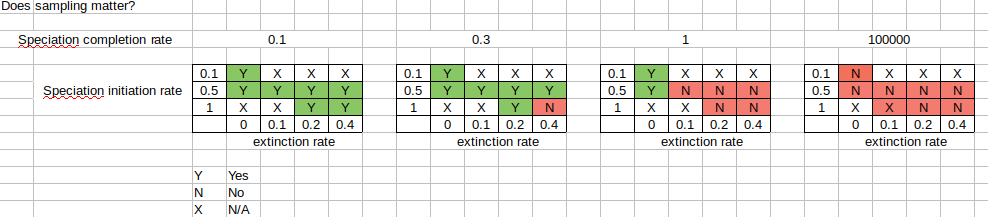
\includegraphics[width=0.9\textwidth]{fig_does_sampling_matter.png}
\end{figure}

\begin{figure}[]
  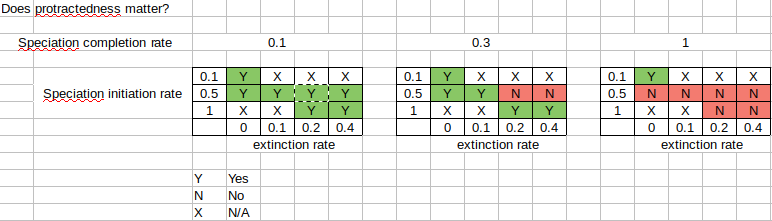
\includegraphics[width=0.9\textwidth]{fig_does_protractedness_matter.png}
\end{figure}

%%%%%%%%%%%%%%%%%%%%%%%%%%%%%%%%%%%%%%%%%%%%%%%%%%%%%%%%%%%%%%%%%%%%%%%%%%%%%%%%%%%%%%
\section{Discussion}
%%%%%%%%%%%%%%%%%%%%%%%%%%%%%%%%%%%%%%%%%%%%%%%%%%%%%%%%%%%%%%%%%%%%%%%%%%%%%%%%%%%%%%


%%%%%%%%%%%%%%%%%%%%%%%%%%%%%%%%%%%%%%%%%%%%%%%%%%%%%%%%%%%%%%%%%%%%%%%%%%%%%%%%%%%%%%
\section{Acknowledgements}
%%%%%%%%%%%%%%%%%%%%%%%%%%%%%%%%%%%%%%%%%%%%%%%%%%%%%%%%%%%%%%%%%%%%%%%%%%%%%%%%%%%%%%

We would like to thank the Center for Information Technology of the University of Groningen for their support
and for providing access to the Peregrine high performance computing cluster.

%%%%%%%%%%%%%%%%%%%%%%%%%%%%%%%%%%%%%%%%%%%%%%%%%%%%%%%%%%%%%%%%%%%%%%%%%%%%%%%%%%%%%%
\section{Authors' contributions}
%%%%%%%%%%%%%%%%%%%%%%%%%%%%%%%%%%%%%%%%%%%%%%%%%%%%%%%%%%%%%%%%%%%%%%%%%%%%%%%%%%%%%%

%%%%%%%%%%%%%%%%%%%%%%%%%%%%%%%%%%%%%%%%%%%%%%%%%%%%%%%%%%%%%%%%%%%%%%%%%%%%%%%%%%%%%%
% Bibliography
%%%%%%%%%%%%%%%%%%%%%%%%%%%%%%%%%%%%%%%%%%%%%%%%%%%%%%%%%%%%%%%%%%%%%%%%%%%%%%%%%%%%%%
% MEE style
\bibliographystyle{mee}
\bibliography{article}
%%%%%%%%%%%%%%%%%%%%%%%%%%%%%%%%%%%%%%%%%%%%%%%%%%%%%%%%%%%%%%%%%%%%%%%%%%%%%%%%%%%%%%

\end{document}
